\documentclass[a4paper,11pt,dvipdfmx]{ujarticle}
% パッケージ
\usepackage{graphicx}
\usepackage{url}
% レイアウト指定を記述したファイルの読み込み
% \input{layout}

% タイトルと氏名を変更せよ．
\title{日本におけるデジタル化の状況}
\author{ G684032026 ISLAM MD RIFATUL}

\begin{document}

\maketitle %ここにタイトルが入る
\section{ブロードバンドの整備状況}
OECDによるブロードバンド回線の普及に関する調査\cite{oecd}によると，
図\ref{fig:broadband}に示すように，日本における
100人あたりの光ファイバー回線の加入者数は29.0で，
韓国，スウェーデン，ノルウェーに続いて第4位になっている．

\begin{figure}[htbp]
  \centering
  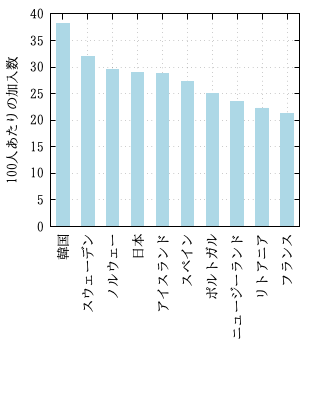
\includegraphics[width=0.7\textwidth]{fig12.png}
  \caption{光ファイバー回線の加入者数（100人あたり）}
  \label{fig:broadband}
\end{figure}
\section{デジタル競争力ランキング}

国際経営開発研究所（IMD）の調査\cite{imd}によると，
日本のデジタル競争力のランキングは表\ref{tbl:ranking}に示すように，
調査対象の64か国中，総合で28位，技術分野で30位となっている．

\begin{table}[htbp]
    \centering
    \caption{デジタル競争力ランキング（64か国中）}
    \label{tbl:ranking}
    \begin{tabular}{|c|c|c|}
        \hline
        国 & 総合 & 技術 \\
        \hline
        米国 & 1位 & 4位 \\
        \hline
        香港 & 2位 & 10位 \\
        \hline
        スウェーデン & 3位 & 8位 \\
        \hline
        デンマーク & 4位 & 2位 \\
        \hline
        シンガポール & 5位 & 3位 \\
        \hline
        韓国 & 12位 & 13位 \\
        \hline
        中国 & 15位 & 20位 \\
        \hline
        日本 & 28位 & 30位 \\
        \hline
    \end{tabular}
\end{table}

\section{考察}

\begin{itemize}
    \item 日本では光ファイバー回線が広く普及しているが，
    韓国などの上位国と比べると，まだ改善できる部分があると考えた．

    \item 日本のデジタル競争力は総合28位であり，
    通信環境だけではなく，技術力や人材育成も重要だと分かった．

    \item 今後はAIやプログラミングを学ぶ人を増やし，
    デジタル技術をもっと活用する必要があると考える．
\end{itemize}
\begin{thebibliography}{9}
\bibitem{oecd}
OECD, \textit{Broadband Statistics}, 2024.
\end{thebibliography}

\end{document}



